% Options for packages loaded elsewhere
\PassOptionsToPackage{unicode}{hyperref}
\PassOptionsToPackage{hyphens}{url}
%
\documentclass[
]{article}
\usepackage{amsmath,amssymb}
\usepackage{lmodern}
\usepackage{ifxetex,ifluatex}
\ifnum 0\ifxetex 1\fi\ifluatex 1\fi=0 % if pdftex
  \usepackage[T1]{fontenc}
  \usepackage[utf8]{inputenc}
  \usepackage{textcomp} % provide euro and other symbols
\else % if luatex or xetex
  \usepackage{unicode-math}
  \defaultfontfeatures{Scale=MatchLowercase}
  \defaultfontfeatures[\rmfamily]{Ligatures=TeX,Scale=1}
\fi
% Use upquote if available, for straight quotes in verbatim environments
\IfFileExists{upquote.sty}{\usepackage{upquote}}{}
\IfFileExists{microtype.sty}{% use microtype if available
  \usepackage[]{microtype}
  \UseMicrotypeSet[protrusion]{basicmath} % disable protrusion for tt fonts
}{}
\makeatletter
\@ifundefined{KOMAClassName}{% if non-KOMA class
  \IfFileExists{parskip.sty}{%
    \usepackage{parskip}
  }{% else
    \setlength{\parindent}{0pt}
    \setlength{\parskip}{6pt plus 2pt minus 1pt}}
}{% if KOMA class
  \KOMAoptions{parskip=half}}
\makeatother
\usepackage{xcolor}
\IfFileExists{xurl.sty}{\usepackage{xurl}}{} % add URL line breaks if available
\IfFileExists{bookmark.sty}{\usepackage{bookmark}}{\usepackage{hyperref}}
\hypersetup{
  pdftitle={HCM SCD risk algorithm cost-effectiveness analysis},
  pdfauthor={Nathan Green, Yang Chen},
  hidelinks,
  pdfcreator={LaTeX via pandoc}}
\urlstyle{same} % disable monospaced font for URLs
\usepackage[margin=1in]{geometry}
\usepackage{longtable,booktabs,array}
\usepackage{calc} % for calculating minipage widths
% Correct order of tables after \paragraph or \subparagraph
\usepackage{etoolbox}
\makeatletter
\patchcmd\longtable{\par}{\if@noskipsec\mbox{}\fi\par}{}{}
\makeatother
% Allow footnotes in longtable head/foot
\IfFileExists{footnotehyper.sty}{\usepackage{footnotehyper}}{\usepackage{footnote}}
\makesavenoteenv{longtable}
\usepackage{graphicx}
\makeatletter
\def\maxwidth{\ifdim\Gin@nat@width>\linewidth\linewidth\else\Gin@nat@width\fi}
\def\maxheight{\ifdim\Gin@nat@height>\textheight\textheight\else\Gin@nat@height\fi}
\makeatother
% Scale images if necessary, so that they will not overflow the page
% margins by default, and it is still possible to overwrite the defaults
% using explicit options in \includegraphics[width, height, ...]{}
\setkeys{Gin}{width=\maxwidth,height=\maxheight,keepaspectratio}
% Set default figure placement to htbp
\makeatletter
\def\fps@figure{htbp}
\makeatother
\setlength{\emergencystretch}{3em} % prevent overfull lines
\providecommand{\tightlist}{%
  \setlength{\itemsep}{0pt}\setlength{\parskip}{0pt}}
\setcounter{secnumdepth}{5}
\ifluatex
  \usepackage{selnolig}  % disable illegal ligatures
\fi
\newlength{\cslhangindent}
\setlength{\cslhangindent}{1.5em}
\newlength{\csllabelwidth}
\setlength{\csllabelwidth}{3em}
\newenvironment{CSLReferences}[2] % #1 hanging-ident, #2 entry spacing
 {% don't indent paragraphs
  \setlength{\parindent}{0pt}
  % turn on hanging indent if param 1 is 1
  \ifodd #1 \everypar{\setlength{\hangindent}{\cslhangindent}}\ignorespaces\fi
  % set entry spacing
  \ifnum #2 > 0
  \setlength{\parskip}{#2\baselineskip}
  \fi
 }%
 {}
\usepackage{calc}
\newcommand{\CSLBlock}[1]{#1\hfill\break}
\newcommand{\CSLLeftMargin}[1]{\parbox[t]{\csllabelwidth}{#1}}
\newcommand{\CSLRightInline}[1]{\parbox[t]{\linewidth - \csllabelwidth}{#1}\break}
\newcommand{\CSLIndent}[1]{\hspace{\cslhangindent}#1}

\title{HCM SCD risk algorithm cost-effectiveness analysis}
\author{Nathan Green, Yang Chen}
\date{09/11/2020}

\begin{document}
\maketitle

\hypertarget{introduction}{%
\subsection{Introduction}\label{introduction}}

Sudden cardiac death (SCD) risk score algorithm details see (O'Mahony et al. 2014).

There have been previous cost-effectiveness analyses of ICD implants (Magnusson and Wimo 2020; Boriani et al. 2014; Bryant et al. 2007; Caro et al. 2007; Cowie et al. 2009; García-Pérez et al. 2015; Mealing et al. 2016; Sanders, Hlatky, and Owens 2005; Smith et al. 2013)

Cost-effectiveness of a cardiovascular risk prediction algorithm.
(Zomer et al. 2017) for statins interventions and people with severe mental illness.

(Yao et al. 2007) use a Markov model and consider multiple implantations attempts if unsuccessful.
(Colquitt et al. 2014) is a Health Technology Assessment which compares optimal pharmacological therapy (OPT) with or without ICD.
(Tomini 2016) is a review of economic evaluation models for cardiac resynchronization therapy with implantable cardioverter defibrillators in patients with heart failure.
(Ommen et al. 2020) 2020 AHA/ACC Guideline for the Diagnosis and Treatment of Patients With Hypertrophic Cardiomyopathy.

\hypertarget{data}{%
\subsection{Data}\label{data}}

The main data set contains individual-level follow-up data of patients with HCM who may have been given an ICD due to some risk decision.
Key cohort characteristics include the following.
Patients were enrolled from the 6 health centres: Athens (474), Bologna (456), Coruna (590), London (1592), Murcia (404), Naples (156); The amount of censoring was 0 (3475), 1 (197); The mean age (sd) was 48 (16); The start of study data collection was in 1972 to 2011. Further plots are given in the Appendix. See (O'Mahony et al. 2014) for further details.

Health and cost data were obtained from literature and expert opinion.
What values we wish to use will determine the form of the state model.
For instance, if cost are only accrued on entry to a state then we may use a tunnel state.
If cost depend on the patient history then we may need to duplicate a state.

Table 1 gives the unit cost and health values used in the model.

\begin{longtable}[]{@{}
  >{\raggedright\arraybackslash}p{(\columnwidth - 8\tabcolsep) * \real{0.37}}
  >{\raggedright\arraybackslash}p{(\columnwidth - 8\tabcolsep) * \real{0.15}}
  >{\raggedright\arraybackslash}p{(\columnwidth - 8\tabcolsep) * \real{0.19}}
  >{\raggedright\arraybackslash}p{(\columnwidth - 8\tabcolsep) * \real{0.09}}
  >{\raggedright\arraybackslash}p{(\columnwidth - 8\tabcolsep) * \real{0.20}}@{}}
\caption{Model parameter values. \(^*\)either one-off/on state entry or recurring.}\tabularnewline
\toprule
Description & Parameter & Value\(^*\) & Range & Source \\
\midrule
\endfirsthead
\toprule
Description & Parameter & Value\(^*\) & Range & Source \\
\midrule
\endhead
\emph{Health} & & & & \\
Manage with ICD & \texttt{u\_icd} & 0.637 QALY/year & & Noyes et al. (2007) \\
Implantation procedure utility & \texttt{u\_implant} & -0.016 & & Smith et al. (2013) \\
Shock utility & \texttt{u\_shock} & -0.5 & & \\
HCM without ICD & \texttt{u\_hcm} & 1 QALY/year & & \\
Death & \texttt{u\_death} & 0 QALY/year & & \\
& & & & \\
\emph{Cost} & & & & \\
ICD appointment & \texttt{c\_appt} & £10 & & \\
Perform risk score & \texttt{c\_rs} & £20? & & \\
Implant ICD & \texttt{c\_implant} & £4,666 & & EY02B Tariffs \\
Implant replacement & \texttt{c\_repl} & £45,000 & & \\
Implant complication & \texttt{c\_compl} & £28,839 & & Smith et al. (2013) \\
Non-fatal shock & \texttt{c\_shock} & £22,880 & & UK Stroke Assoc. \\
HCM without ICD & \texttt{c\_hcm} & 0 & & \\
SCD & \texttt{c\_scd} & 0 & & \\
All-cause death & \texttt{c\_death} & 0 & & \\
& & & & \\
\emph{Probabilities} & & & & \\
Initial implant complication & \texttt{p\_compl} & 0.047 & & Smith et al. (2013) \\
Replacement implant complication & \texttt{p\_repl} & 0.032 & & Smith et al. (2013) \\
& & & & \\
Time horizon & \texttt{T} & 12 years & & \\
Implant replacement & \texttt{t\_repl} & 10 years & & \\
Annual number of appointments & n\_appt & 2 & & \\
\bottomrule
\end{longtable}

Table 2 gives the starting state populations for non-zero states.

\begin{longtable}[]{@{}
  >{\raggedright\arraybackslash}p{(\columnwidth - 4\tabcolsep) * \real{0.25}}
  >{\raggedright\arraybackslash}p{(\columnwidth - 4\tabcolsep) * \real{0.14}}
  >{\raggedright\arraybackslash}p{(\columnwidth - 4\tabcolsep) * \real{0.18}}@{}}
\caption{Starting state populations by decision rule.}\tabularnewline
\toprule
Risk rule & State & Population \\
\midrule
\endfirsthead
\toprule
Risk rule & State & Population \\
\midrule
\endhead
Observed & HCM ICD & 559 \\
- & HCM & 3113 \\
Score \textgreater{} 4\% & HCM ICD & 2561 \\
- & HCM & 1111 \\
Score \textgreater{} 6\% & HCM ICD & 542 \\
- & HCM & 3130 \\
Risk factor \textgreater0 & HCM ICD & 1785 \\
- & HCM & 1887 \\
Risk factor \textgreater1 & HCM ICD & 481 \\
- & HCM & 3191 \\
Risk factor \textgreater2 & HCM ICD & 78 \\
- & HCM & 3594 \\
\bottomrule
\end{longtable}

\hypertarget{methods}{%
\subsection{Methods}\label{methods}}

The individual-level patient data are first stratified in to two groups for each risk algorithm.
These are

\begin{itemize}
\tightlist
\item
  Partition observed in data set
\item
  ICD given if number of risk factors \textgreater{} 0, 1 or 2
\item
  ICD given if risk score \textgreater{} 6\%
\item
  ICD given if risk score \textgreater{} 4\%
\end{itemize}

We included the option of a fuzzy decision boundary such that near the threshold there is some random variation as to whether a patient received an ICD or not.

\hypertarget{markov-model}{%
\subsubsection{Markov model}\label{markov-model}}

Th patient data give us starting state populations for HCM with ICD and HCM without ICD which will be different for each risk decision rule.
Further, the transition probabilities from these states will differ because of the case mixes.

A diagram of the current cohort model is given in Figure \ref{fig:model}.

\begin{figure}

{\centering 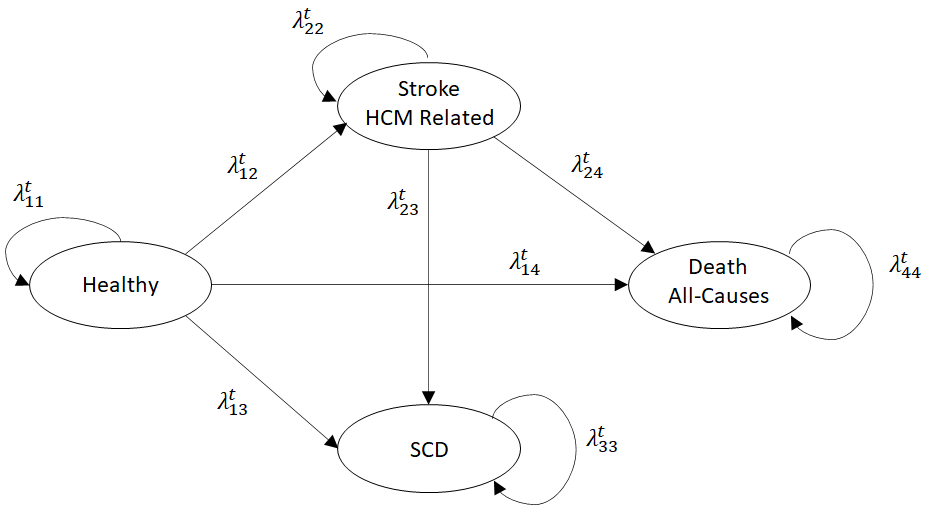
\includegraphics[width=3.25in]{../../images/model_diagram} 

}

\caption{Markov model diagram. Bold circles represent starting states and dashed circles represent sink states.}\label{fig:model}
\end{figure}

Assuming that shocked patients return to the HCM ICD state then the transition matrix looks like the following.

\[
\begin{pmatrix}
p_{11} & p_{12} & 0 & 0 & p_{15}\\
1 & 0 & 0 & 0 & 0\\
0 & 0 & p_{33} & p_{34} & p_{35}\\
0 & 0 & 0 & 1 & 0\\
0 & 0 & 0 & 0 & 1
\end{pmatrix}
\]

We have used a year step size but if e.g.~cost are accrued at different intervals then this can be adapted.
The time horizon is set at 12 years from time of implant.

\hypertarget{state-health-and-cost-equations}{%
\subsubsection{State health and cost equations}\label{state-health-and-cost-equations}}

We assume that an ICD patient has 2 annual appointments.
All shocks are treated the same in terms of costs and health impact.
Implantation can have complications.
The cost of an implant complication is taken as a weighted sum of infection and dislodgement cost with values from (Smith et al. 2013).
Subscript \(s\) denotes the state number and superscript denotes the intervention either ICD or not.

\begin{itemize}
\tightlist
\item
  Annual health: \[
  e^0_{s=1}(t) = e^1_{s=1}(t) = \mbox{u\_hcm} + \mbox{u\_icd}
  \] \[
  e^0_{s=3}(t) = e^1_{s=3}(t) = \mbox{u\_hcm}
  \] \[
  e^0_{s=2}(t) = e^1_{s=2}(t) = \mbox{u\_shock}
  \]
\end{itemize}

\[
e^0_{s}(t) = e^1_{s}(t) = 0, \;\; s = 4,5,6
\]

\begin{itemize}
\tightlist
\item
  Initial costs: \[
  c^0_{s=1}(t = 0) = \mbox{c\_icd} + \mbox{p\_compl} \times \mbox{c\_compl}
  \]
\end{itemize}

\[
c^1_{s=1}(t = 0) = \mbox{c\_icd} + \mbox{c\_rscore} + \mbox{p\_compl} \times \mbox{c\_compl}
\]

\begin{itemize}
\tightlist
\item
  Annual cost: \[
  c^0_{s=1}(t) = c^1_{s=1}(t) = 2 \mbox{c\_appt}, \;\; t \neq \mbox{t\_repl}
  \]
\end{itemize}

\[
c^0_{s=2}(t) = c^1_{s=2}(t) = \mbox{c\_shock}
\]

\begin{itemize}
\tightlist
\item
  Implant replacement cost \[
  c^0_{s=1}(t) = c^1_{s=1}(t) = 2 \mbox{c\_appt} + \mbox{c\_repl} + \mbox{p\_compl} \times \mbox{c\_compl}, \;\;  t = \mbox{t\_repl}
  \]
\end{itemize}

\hypertarget{transition-probability-inference}{%
\paragraph{Transition probability inference}\label{transition-probability-inference}}

Using WinBUGS (Zhang 2014) called from R, each new data set is used to generate posterior samples of transition probabilities.
Denote \(x\) as the observed number of transitions, \(p\) the probability of a transition and \(n\) as the total number of transitions from a given state.
The hyperparameters \(\alpha\) characterise the prior knowledge on \(p\).
Superscripts indicate the decision rule used.

\[x^{(1)}_{i.} \sim \mbox{Multinomial}(p^{(1)}_{i.}, n^{(1)}_i), \;\; i = 1,3\]

\[x^{(2)}_{i.} \sim \mbox{Multinomial}(p^{(2)}_{i.}, n^{(2)}_i), \;\; i = 1,3\]

\[p^{(1)}_{i.} \sim \mbox{Dirichlet}(\boldsymbol{\alpha}^{(1)} ), \;\; i = 1,3\]

\[p^{(2)}_{i.} \sim \mbox{Dirichlet}(\boldsymbol{\alpha}^{(2)} ), \;\; i = 1,3\]

For all sink states,

\[
p^{(s)}_{ij} = \left\{
\begin{array}{ll}
1 & \mbox{if $i = j$};\\
0 & \mbox{if $i \neq j$}.
\end{array} \right.
\]

\hypertarget{results}{%
\subsection{Results}\label{results}}

We give results of the model fitting and cost-effectiveness analysis.

\hypertarget{model-fitting}{%
\subsubsection{Model fitting}\label{model-fitting}}

Figures \ref{fig:histnoICD} and \ref{fig:histICD} give histograms of posterior distributions for state transition probabilities for no groups without and with ICD implants.

\begin{figure}

{\centering 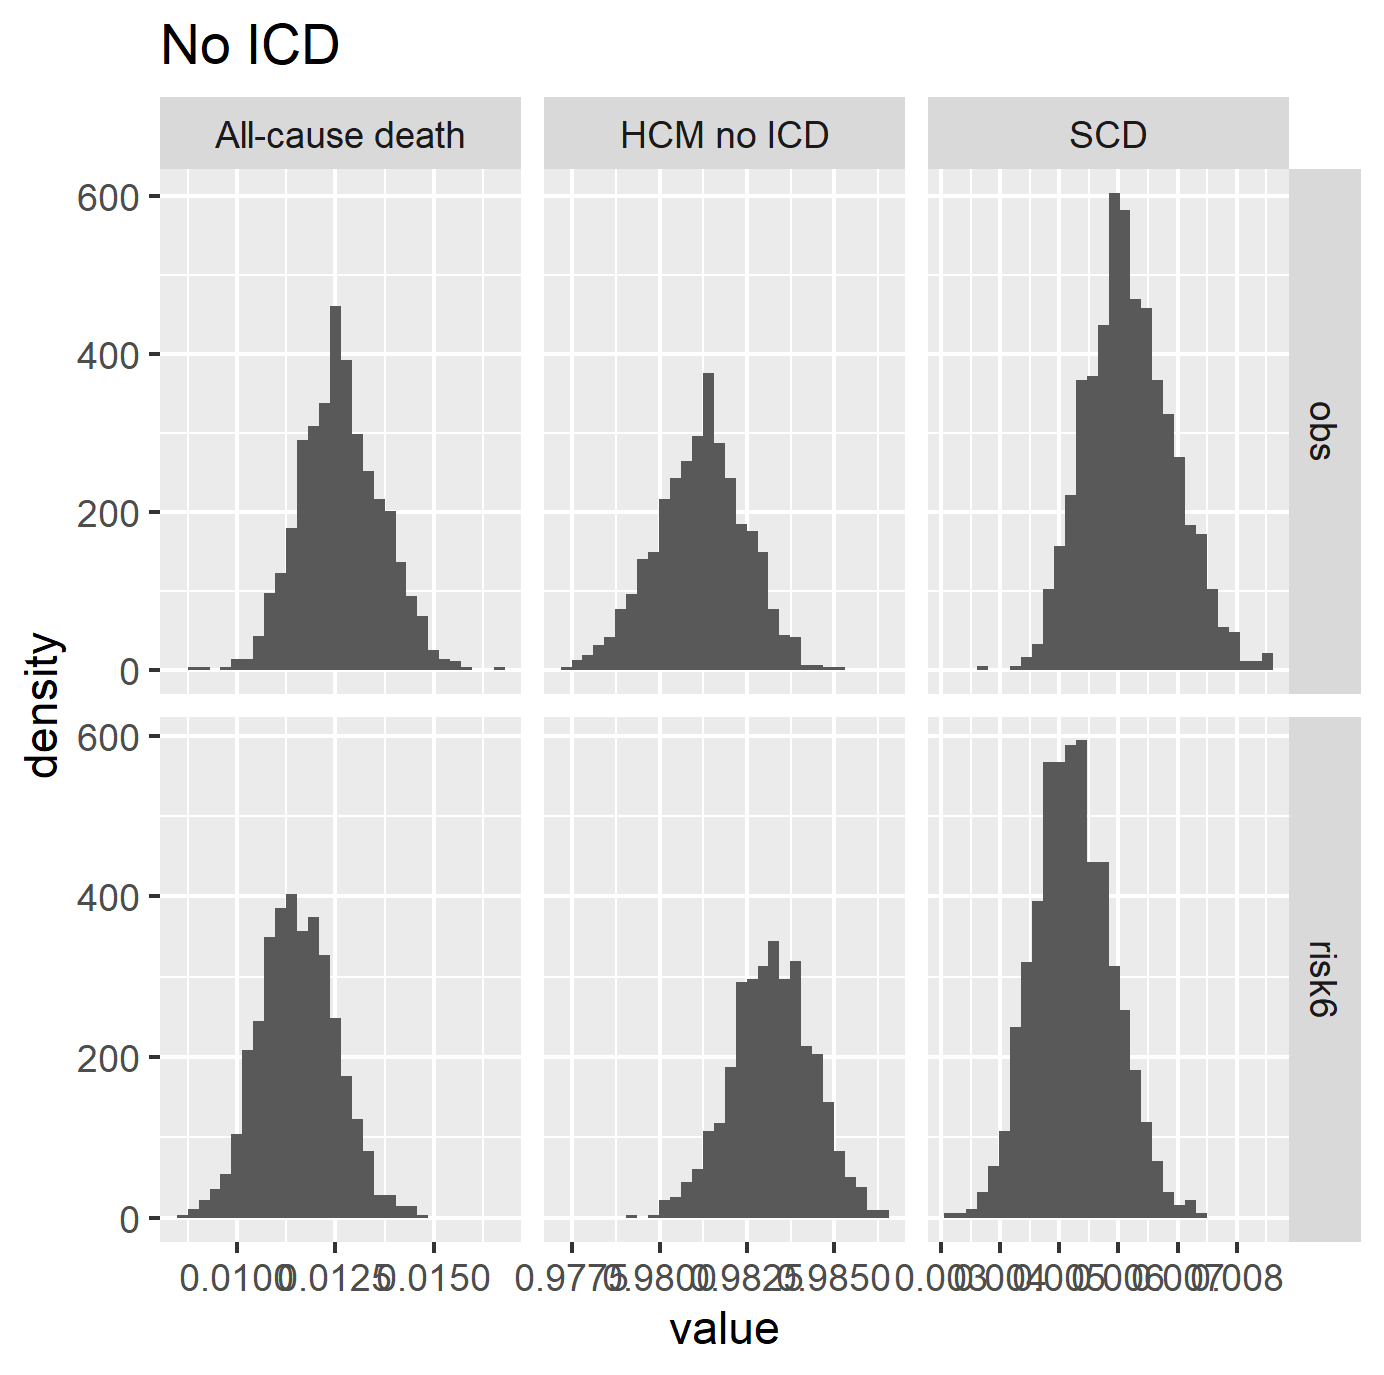
\includegraphics[width=0.8\linewidth]{../../images/post_hist_noICD} 

}

\caption{Histogram of posterior distributions for state transition probabilities.}\label{fig:histnoICD}
\end{figure}

\begin{figure}

{\centering 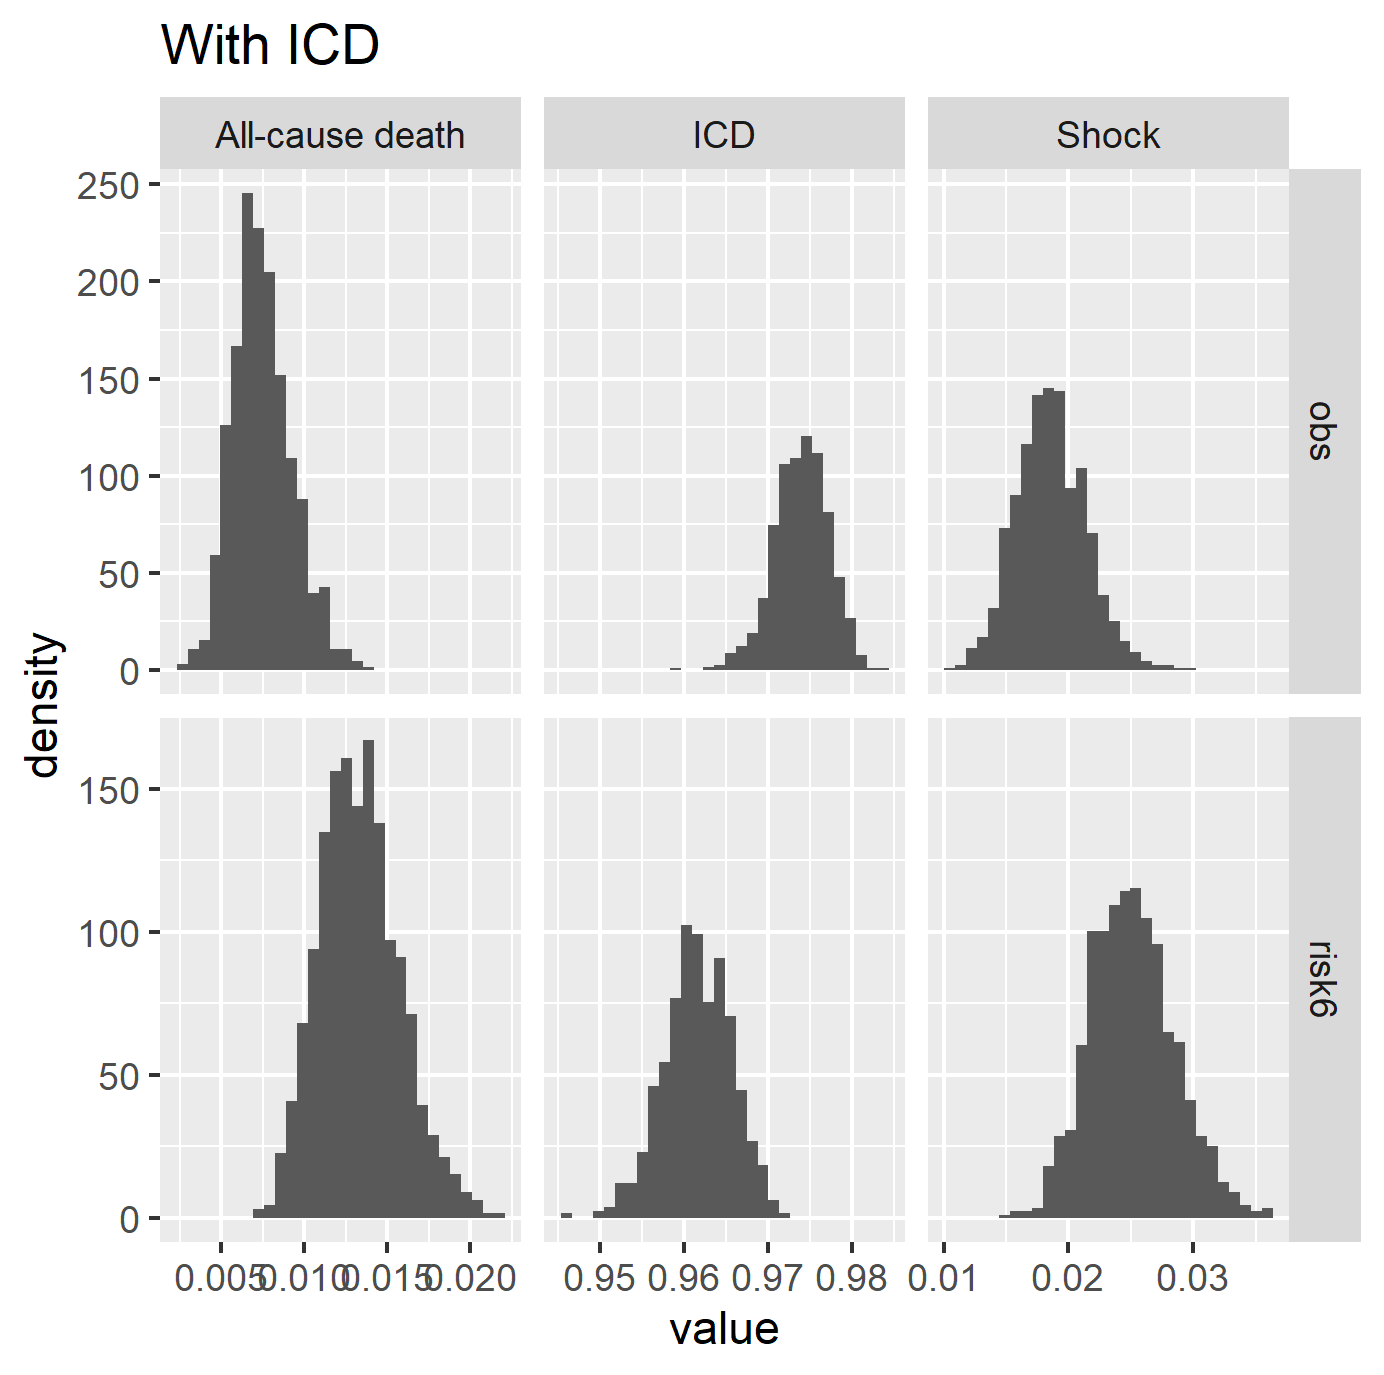
\includegraphics[width=0.8\linewidth]{../../images/post_hist_withICD} 

}

\caption{Histogram of posterior distributions for state transition probabilities.}\label{fig:histICD}
\end{figure}

Figure \ref{fig:statepop} gives an example of state occupancy over time plot.
This shows that for the new algorithm there are fewer SCD and more shocks.

\begin{figure}

{\centering 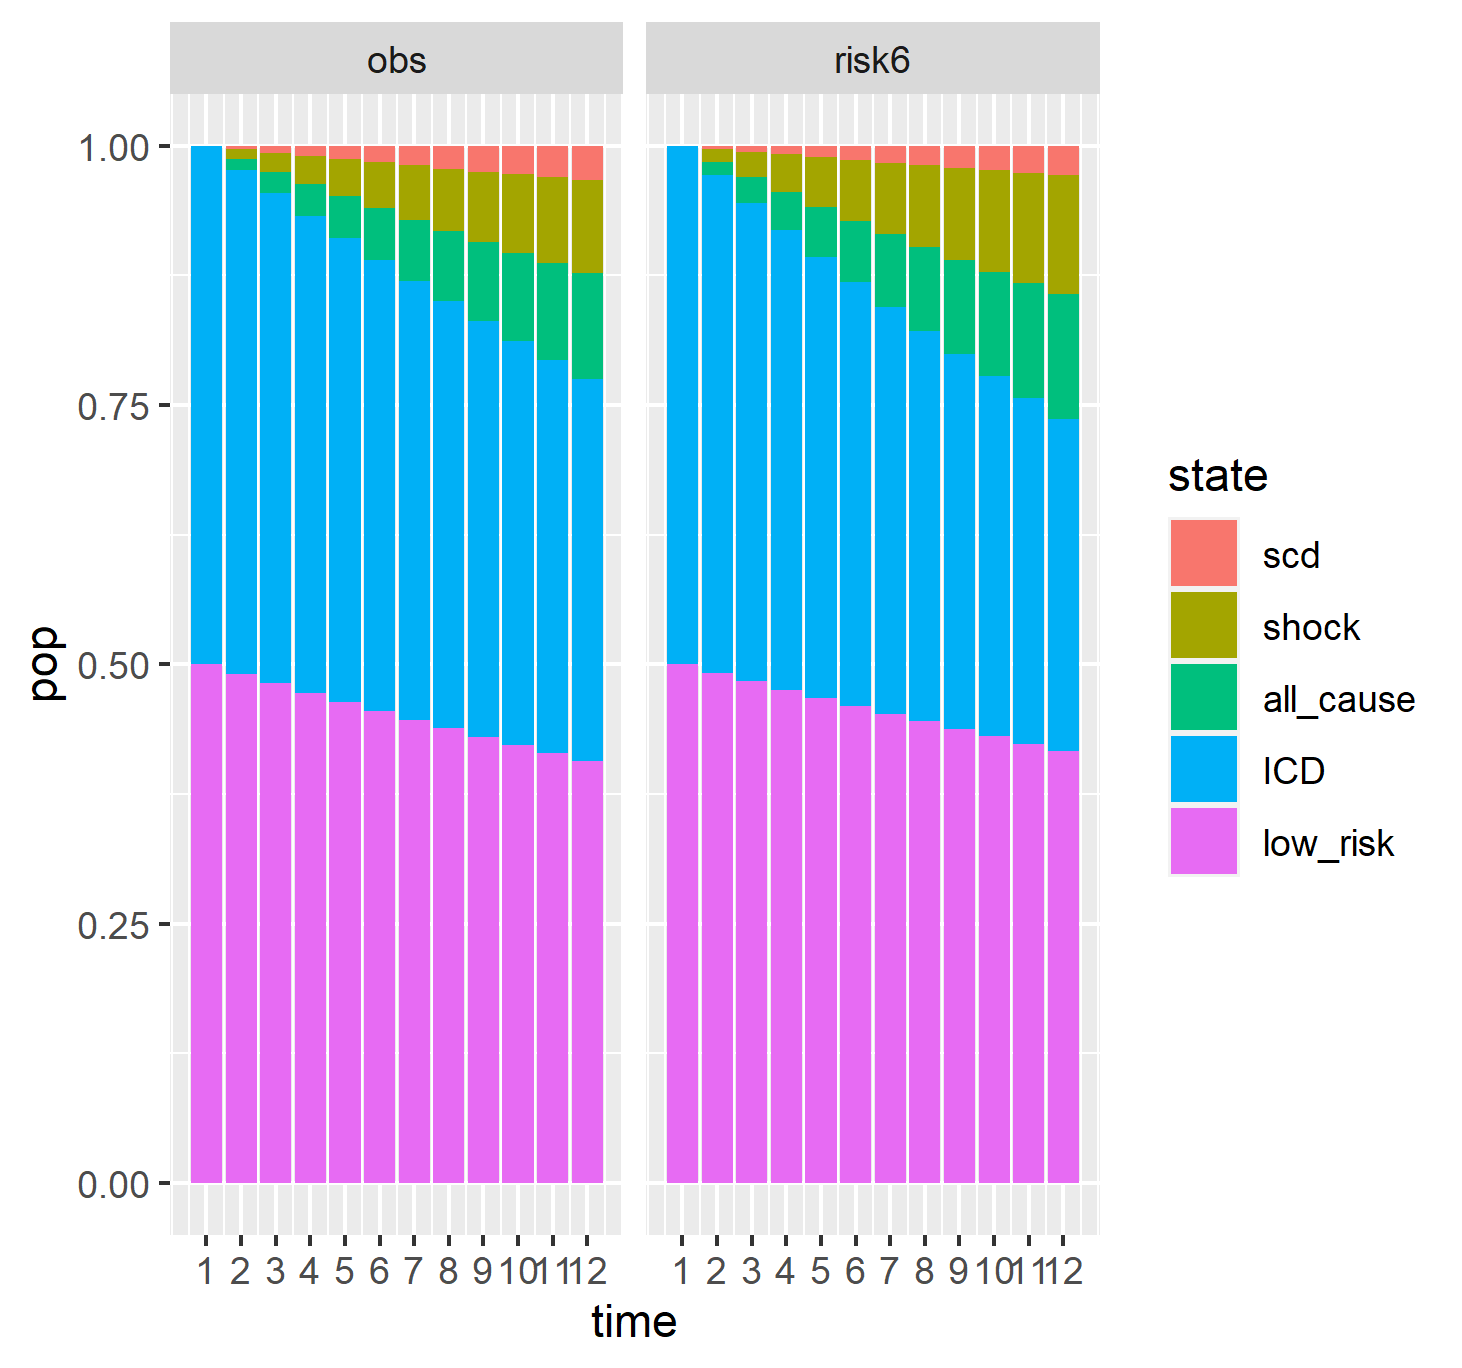
\includegraphics[width=20.31in]{../../images/state_pop_over_time} 

}

\caption{State occupancy over time.}\label{fig:statepop}
\end{figure}

\hypertarget{cost-effectiveness}{%
\subsubsection{Cost-effectiveness}\label{cost-effectiveness}}

\begin{longtable}[]{@{}llllll@{}}
\caption{Cost-effectiveness statistics}\tabularnewline
\toprule
Strategy & Cost, \(c\) & \(\Delta c\) & QALYs, \(e\) & \(\Delta e\) & ICER \\
\midrule
\endfirsthead
\toprule
Strategy & Cost, \(c\) & \(\Delta c\) & QALYs, \(e\) & \(\Delta e\) & ICER \\
\midrule
\endhead
Baseline & & & & & \\
\textgreater{} 4\% & & & & & \\
\textgreater{} 6\% & & & & & \\
\textgreater{} 1 risk factor & & & & & \\
\textgreater{} 2 risk factors & & & & & \\
\bottomrule
\end{longtable}

Figure \ref{fig:ceac} gives the CEAC and
Figure \ref{fig:ceplane} gives the CE-plane.

\begin{figure}

{\centering 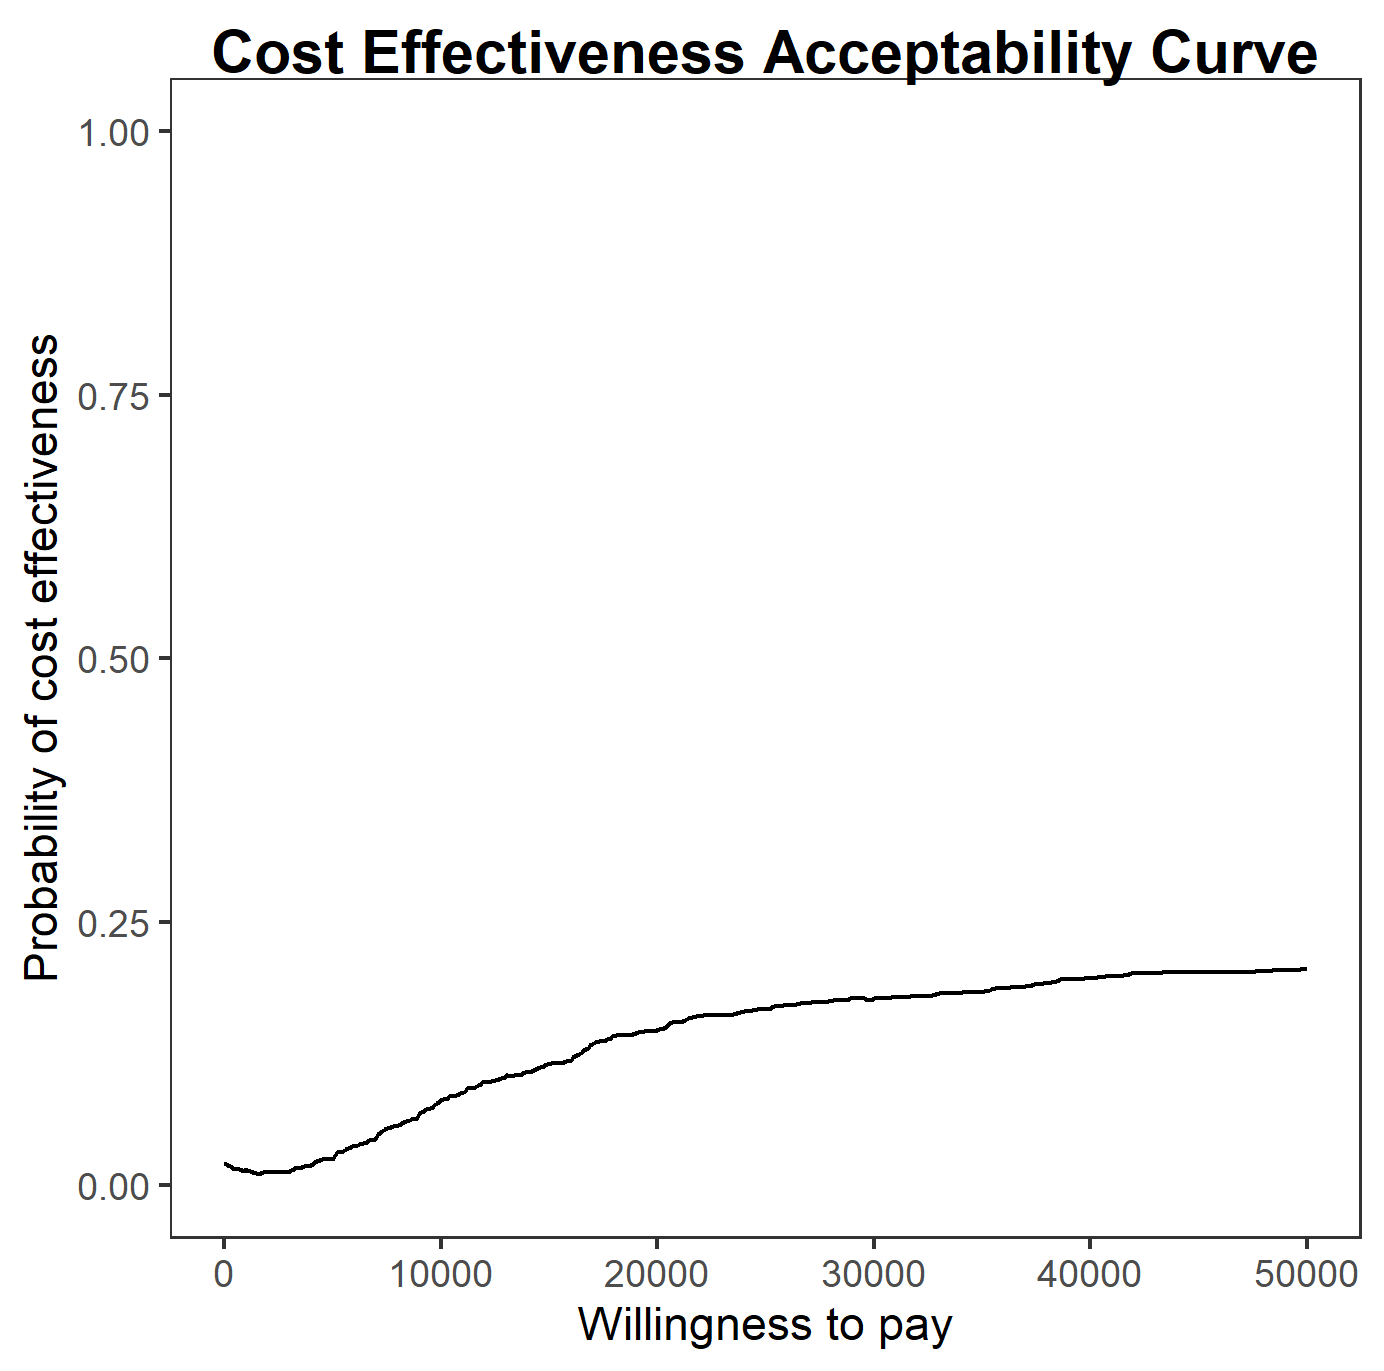
\includegraphics[width=19.22in]{../../images/ceac} 

}

\caption{Cost-effectiveness acceptability curve (CEAC).}\label{fig:ceac}
\end{figure}

\begin{figure}

{\centering 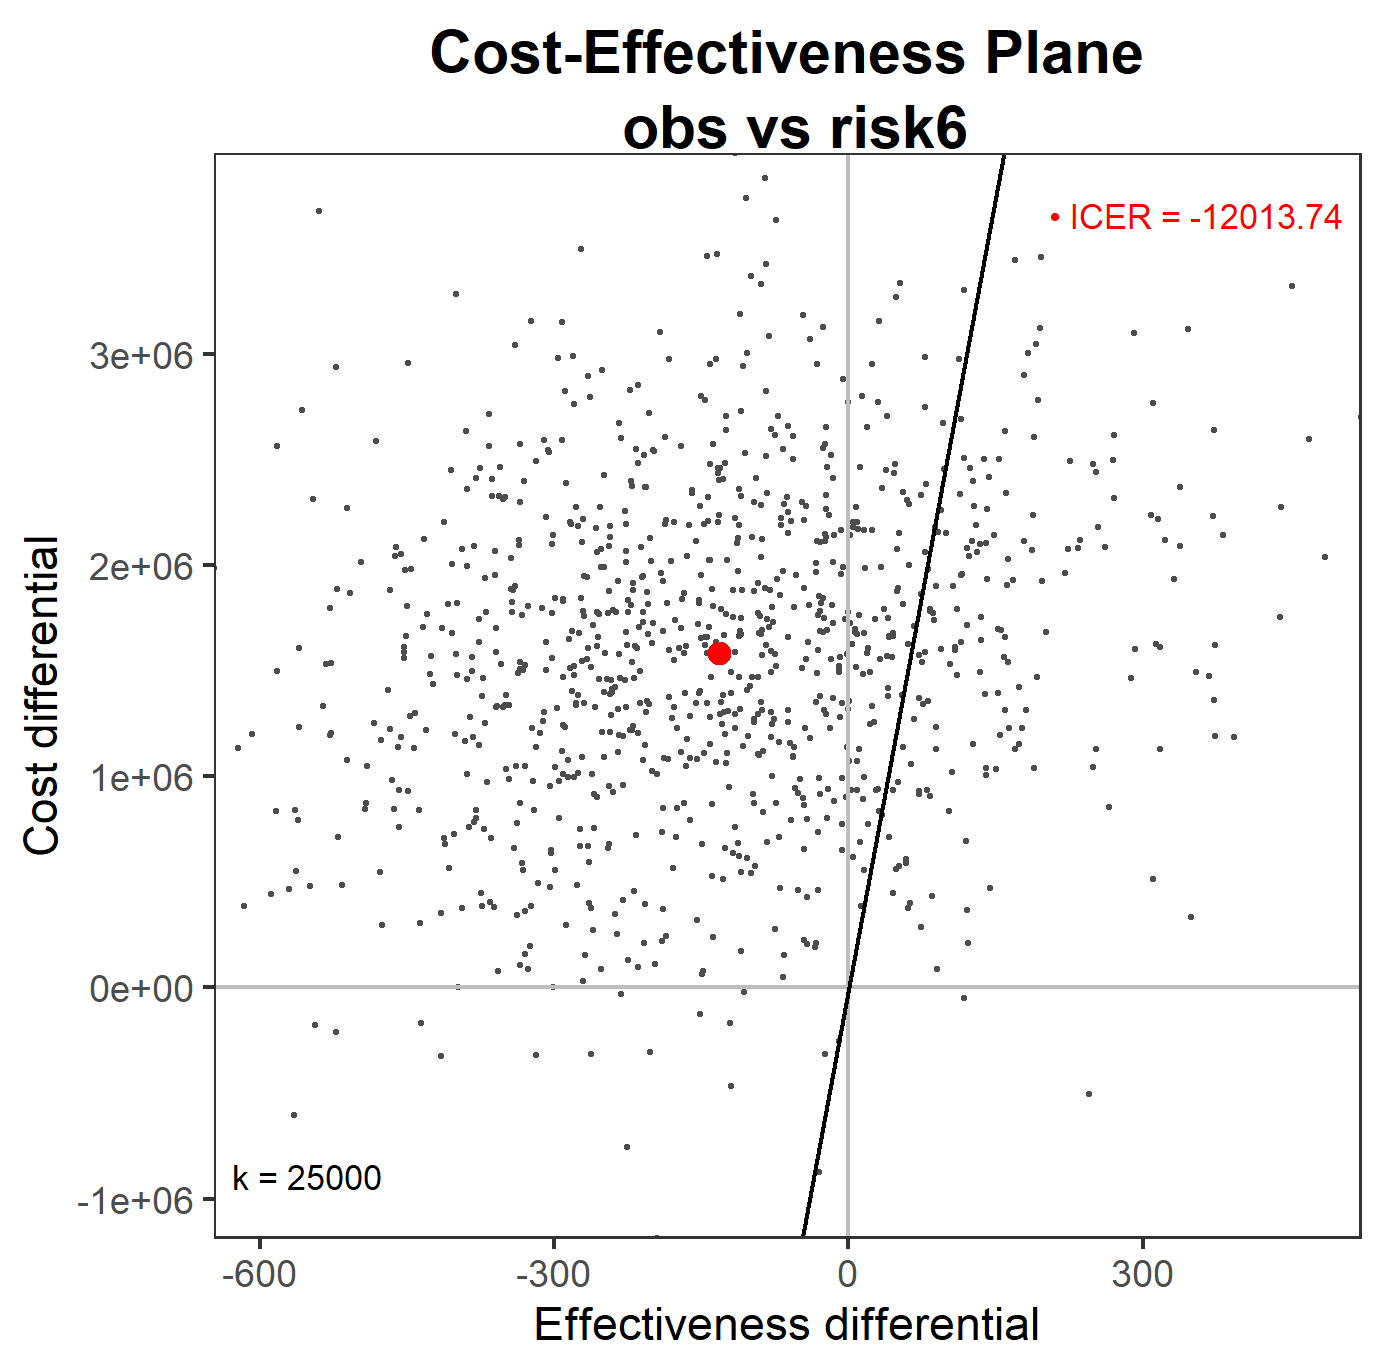
\includegraphics[width=19.22in]{../../images/ceplane} 

}

\caption{Cost-effectiveness plane.}\label{fig:ceplane}
\end{figure}

\hypertarget{discussion}{%
\subsection{Discussion}\label{discussion}}

Decision making as to whether have the implant is shared between patient and medical professional.
The SCD risk score is a support tool which contributes to the final decision.
An SCD risk score of 6\% is treatment recommendation for one patient versus another.
There could be individual preferences that out-weighs the risk score and mean a patient chooses the alternative.

Having more robust quality of life data will help to make such decisions.
more embedded PROMs research

Informatics Consult (Lai et al. 2021) automation to scale evidence generation and to accelerate the return of results within clinical time-scales.

We did not include CRT-D or s-ICD but that can be overcome by sensitivity analyses that show e.g.~the main message is that conclusions about the ICER etc will be robust to most departures from base assumptions other than tweaks in utility (which are the part of the model based on the weakest data!)

(Olivotto et al. 2020) The role of new DMARDs and their ability to influence quality of life.
So if both ICD and non-ICD patients experience significant increases in QoL, are these equally distributed?

\hypertarget{appendix}{%
\section{Appendix}\label{appendix}}

\begin{figure}

{\centering 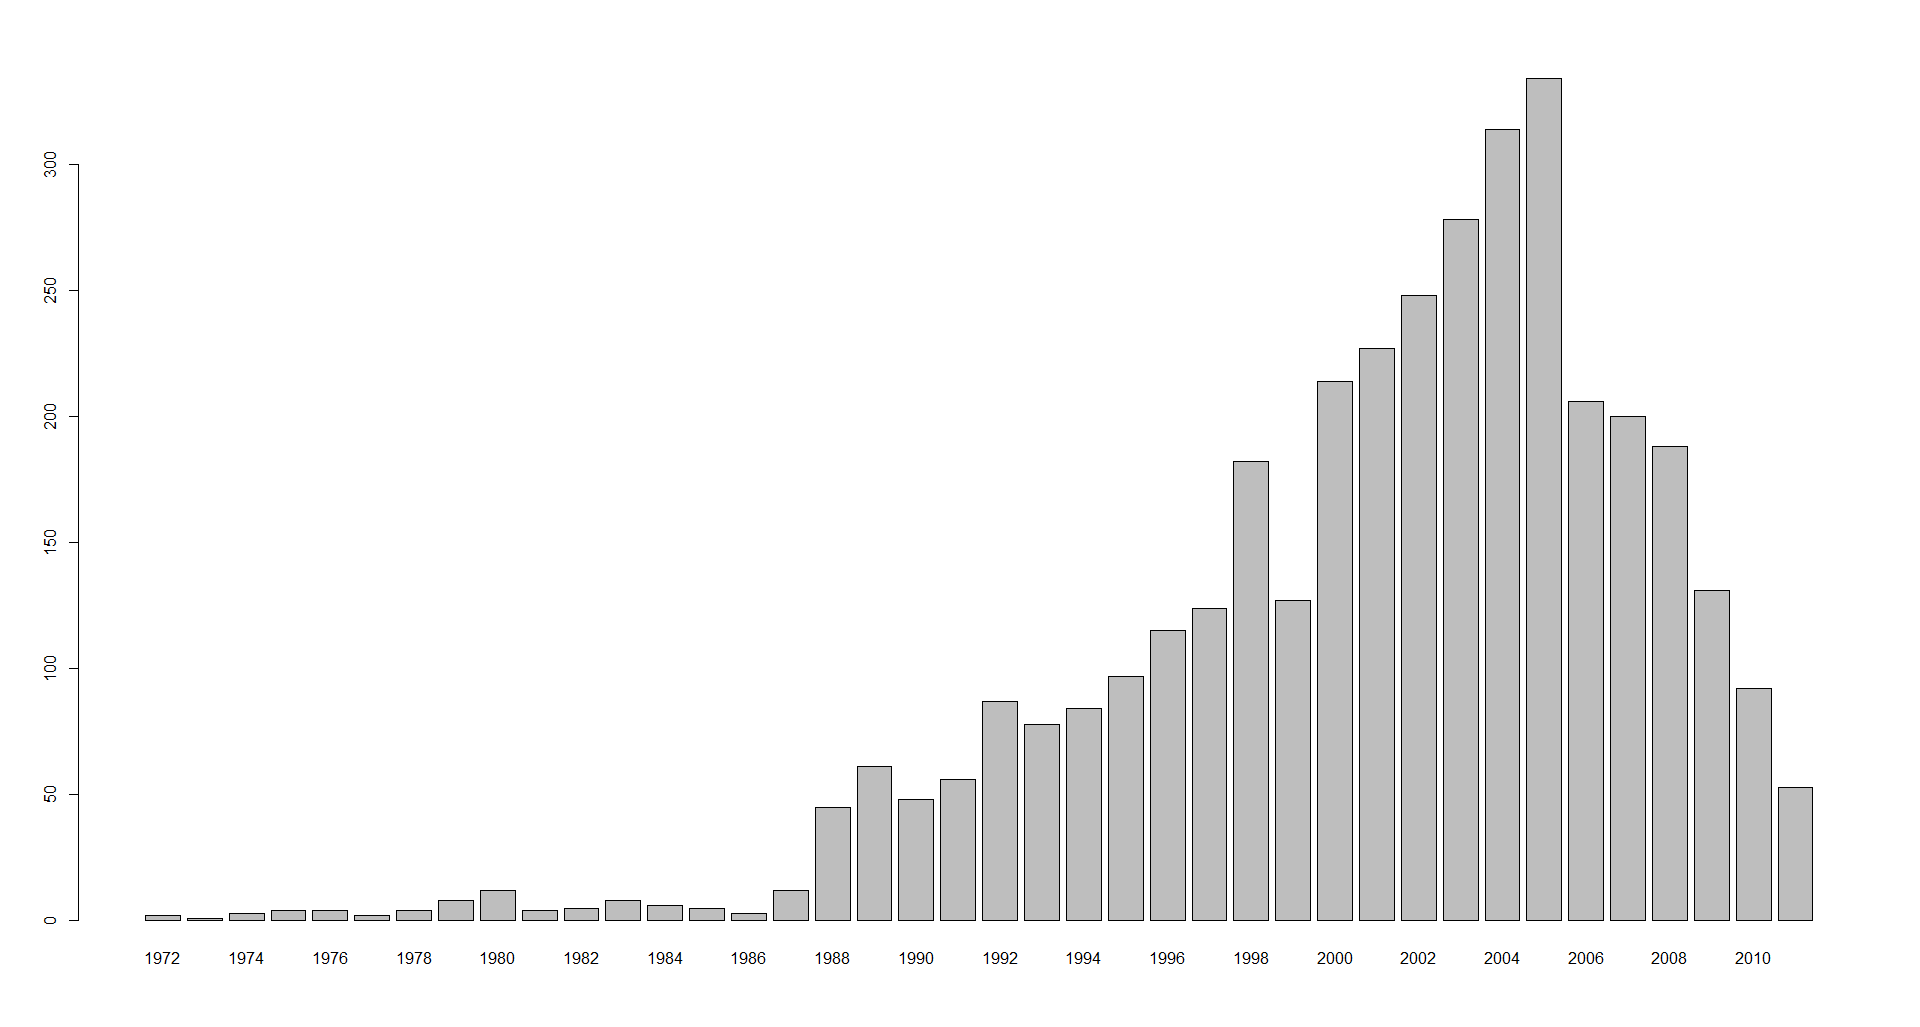
\includegraphics[width=0.8\linewidth]{../../images/year_of_entry_barplot} 

}

\caption{Year of study entry bar plot.}\label{fig:barplot}
\end{figure}

\hypertarget{references}{%
\section*{References}\label{references}}
\addcontentsline{toc}{section}{References}

\hypertarget{refs}{}
\begin{CSLReferences}{1}{0}
\leavevmode\hypertarget{ref-Boriani2014}{}%
Boriani, Giuseppe, Paolo Cimaglia, Mauro Biffi, Cristian Martignani, Matteo Ziacchi, Cinzia Valzania, and Igor Diemberger. 2014. {``{Cost-effectiveness of implantable cardioverter-defibrillator in today's world}.''} \emph{Indian Heart Journal} 66 (SUPPL. 1): S101--4. \url{https://doi.org/10.1016/j.ihj.2013.12.034}.

\leavevmode\hypertarget{ref-Bryant2007}{}%
Bryant, Jackie, Hakan Brodin, Emma Loveman, and Andrew Clegg. 2007. {``{Clinical effectiveness and cost-effectiveness of implantable cardioverter defibrillators for arrhythmias: A systematic review and economic evaluation}.''} \emph{International Journal of Technology Assessment in Health Care} 23 (1): 63--70. \url{https://doi.org/10.1017/S0266462307051586}.

\leavevmode\hypertarget{ref-Caro2007}{}%
Caro, J. Jaime, Alexandra Ward, H. Baris Deniz, Judith A. O'Brien, and Jenifer L. Ehreth. 2007. {``{Cost-benefit analysis of preventing sudden cardiac deaths with an implantable cardioverter defibrillator versus amiodarone}.''} \emph{Value in Health} 10 (1): 13--22. \url{https://doi.org/10.1111/j.1524-4733.2006.00140.x}.

\leavevmode\hypertarget{ref-Colquitt2014}{}%
Colquitt, Jill L, Diana Mendes, Andrew J Clegg, Petra Harris, Keith Cooper, Joanna Picot, and Jackie Bryant. 2014. {``{Implantable cardioverter defibrillators for the treatment of arrhythmias and cardiac resynchronisation therapy for the treatment of heart failure: systematic review and economic evaluation}.''} \emph{Health Technology Assessment} 18 (56). \url{https://doi.org/10.3310/hta18560}.

\leavevmode\hypertarget{ref-Cowie2009}{}%
Cowie, Martin R., Deborah Marshall, Michael Drummond, Nicole Ferko, Michael Maschio, Matthias Ekman, Luc De Roy, et al. 2009. {``{Lifetime cost-effectiveness of prophylactic implantation of a cardioverter defibrillator in patients with reduced left ventricular systolic function: Results of markov modelling in a european population}.''} \emph{Europace} 11 (6): 716--26. \url{https://doi.org/10.1093/europace/eup068}.

\leavevmode\hypertarget{ref-Garcia-Perez2015}{}%
García-Pérez, Lidia, Pilar Pinilla-Domínguez, Antonio García-Quintana, Eduardo Caballero-Dorta, F. Javier García-García, Renata Linertová, and Iñaki Imaz-Iglesia. 2015. {``{Economic evaluations of implantable cardioverter defibrillators: a systematic review}.''} \emph{European Journal of Health Economics} 16 (8): 879--93. \url{https://doi.org/10.1007/s10198-014-0637-x}.

\leavevmode\hypertarget{ref-Lai2021}{}%
Lai, Alvina G, Wai Hoong Chang, Constantinos A Parisinos, Michail Katsoulis, M Ruth, Anoop D Shah, Vincent Nguyen, et al. 2021. {``{An Informatics Consult approach for generating clinical evidence for treatment decisions}.''} \emph{medRxiv}. https://doi.org/\url{https://doi.org/10.1101/2021.01.10.21249331}.

\leavevmode\hypertarget{ref-Magnusson2020}{}%
Magnusson, Peter, and Anders Wimo. 2020. {``{Health economic evaluation of implantable cardioverter defibrillators in hypertrophic cardiomyopathy in adults}.''} \emph{International Journal of Cardiology} 311: 46--51. \url{https://doi.org/10.1016/j.ijcard.2020.02.055}.

\leavevmode\hypertarget{ref-Mealing2016}{}%
Mealing, Stuart, Beth Woods, Neil Hawkins, Martin R. Cowie, Christopher J. Plummer, William T. Abraham, John F. Beshai, Helmut Klein, and Mark Sculpher. 2016. {``{Cost-effectiveness of implantable cardiac devices in patients with systolic heart failure}.''} \emph{Heart} 102 (21): 1742--49. \url{https://doi.org/10.1136/heartjnl-2015-308883}.

\leavevmode\hypertarget{ref-Noyes2007}{}%
Noyes, Katia, Ethan Corona, Jack Zwanziger, W. Jackson Hall, Hongwei Zhao, Hongkun Wang, Arthur J. Moss, and Andrew W. Dick. 2007. {``{Health-related quality of life consequences of implantable cardioverter defibrillators: Results from MADIT II}.''} \emph{Medical Care} 45 (5): 377--85. \url{https://doi.org/10.1097/01.mlr.0000257142.12600.c1}.

\leavevmode\hypertarget{ref-OMahony2014}{}%
O'Mahony, Constantinos O, Fatima Jichi, Menelaos Pavlou, Lorenzo Monserrat, Aristides Anastasakis, Claudio Rapezzi, Elena Biagini, et al. 2014. {``{Myocardial disease A novel clinical risk prediction model for sudden cardiac death in hypertrophic cardiomyopathy (HCM Risk-SCD)}.''} \emph{European Heart Journal} 35: 2010--20. \url{https://doi.org/10.1093/eurheartj/eht439}.

\leavevmode\hypertarget{ref-Olivotto2020}{}%
Olivotto, Iacopo, Artur Oreziak, Roberto Barriales-Villa, Theodore P. Abraham, Ahmad Masri, Pablo Garcia-Pavia, Sara Saberi, et al. 2020. {``{Mavacamten for treatment of symptomatic obstructive hypertrophic cardiomyopathy (EXPLORER-HCM): a randomised, double-blind, placebo-controlled, phase 3 trial}.''} \emph{The Lancet} 396 (10253): 759--69. \url{https://doi.org/10.1016/S0140-6736(20)31792-X}.

\leavevmode\hypertarget{ref-Ommen2020}{}%
Ommen, Steve R., Seema Mital, Michael A. Burke, Sharlene M. Day, Anita Deswal, Perry Elliott, Lauren L. Evanovich, et al. 2020. {``{2020 AHA/ACC Guideline for the Diagnosis and Treatment of Patients With Hypertrophic Cardiomyopathy}.''} \emph{Circulation} 142 (25). \url{https://doi.org/10.1161/cir.0000000000000937}.

\leavevmode\hypertarget{ref-Sanders2005}{}%
Sanders, Gillian D, Mark A Hlatky, and Douglas K Owens. 2005. {``{Cost-Effectiveness of Implantable Cardioverter--Defibrillators},''} 1471--80.

\leavevmode\hypertarget{ref-Smith2013}{}%
Smith, Tim, Luc Jordaens, Dominic A. M. J. Theuns, Pascal F. Van Dessel, Arthur A. Wilde, and M. G. Myriam Hunink. 2013. {``{The cost-effectiveness of primary prophylactic implantable defibrillator therapy in patients with ischaemic or non-ischaemic heart disease: A European analysis}.''} \emph{European Heart Journal} 34 (3): 211--19. \url{https://doi.org/10.1093/eurheartj/ehs090}.

\leavevmode\hypertarget{ref-Tomini2016}{}%
Tomini, F. 2016. {``{A review of economic evaluation models for cardiac resynchronization therapy with implantable cardioverter defibrillators in patients with heart failure}.''} \emph{Eur J Health Econ}, 1159--72. \url{https://doi.org/10.1007/s10198-015-0752-3}.

\leavevmode\hypertarget{ref-Yao2007}{}%
Yao, Guiqing, Nick Freemantle, Melanie J Calvert, Stirling Bryan, Jean-claude Daubert, and John G F Cleland. 2007. {``{The long-term cost-effectiveness of cardiac resynchronization therapy with or without an implantable cardioverter-defibrillator}.''} \emph{European Heart Journal}, 42--51. \url{https://doi.org/10.1093/eurheartj/ehl382}.

\leavevmode\hypertarget{ref-Zhang2014}{}%
Zhang, Zhiyong. 2014. {``{WebBUGS: Conducting Bayesian statistical analysis online}.''} \emph{Journal of Statistical Software} 61 (7): 1--30. \url{https://doi.org/10.18637/jss.v061.i07}.

\leavevmode\hypertarget{ref-Zomer2017}{}%
Zomer, Ella, David Osborn, Irwin Nazareth, Ruth Blackburn, Alexandra Burton, Sarah Hardoon, Richard Ian, et al. 2017. {``{Effectiveness and cost-effectiveness of a cardiovascular risk prediction algorithm for people with severe mental illness ( PRIMROSE )}.''} \emph{BMJ Open}, 1--11. \url{https://doi.org/10.1136/bmjopen-2017-018181}.

\end{CSLReferences}

\end{document}
